\section{The Isomorphism Theorems}

Let $G$ be a group.

\Exercise1 Let $F$ be a finite field of order $q$ and let
$n\in\Z^+$. Prove that
\begin{equation*}
  \ord{GL_n(F):SL_n(F)} = q - 1.
\end{equation*}
\begin{proof}
  In Exercise~\ref{exercise:quotient-group:GL-mod-SL} we saw that
  $GL_n(F)/SL_n(F)\cong F^\times$. Therefore
  \begin{equation*}
    \ord{GL_n(F):SL_n(F)}
    = \ord{GL_n(F)/SL_n(F)}
    = \ord{F^\times}
    = q - 1,
  \end{equation*}
  since $F^\times$ consists of all members of $F$ excluding the $0$
  element.
\end{proof}

\Exercise2 Prove all parts of the Lattice Isomorphism Theorem.
\begin{proof}
  First we show that there is a bijection from the set $\mathcal{A}$
  of subgroups $A$ of $G$ containing $N$ onto the set
  $\overline{\mathcal{A}}$ of subgroups $\overline{A} = A/N$ of
  $G/N$. Let $\pi\colon G\to G/N$ be the natural projection of $G$
  onto $G/N$. Then define the map
  $\Phi\colon\mathcal{A}\to\overline{\mathcal{A}}$ by
  \begin{equation*}
    \Phi(A) = \pi(A) = \{aN \mid a\in A\}.
  \end{equation*}
  That $\Phi(A)\leq G/N$ for any $A\leq G$ is easy to check: $\Phi(A)$
  is nonempty since it includes $1N$, and if $a,b\in A$, then
  \begin{equation*}
    (aN)(bN)^{-1} = (ab^{-1})N\in\Phi(A).
  \end{equation*}

  To show $\Phi$ is injective, suppose $\Phi(A) = \Phi(B)$. Let
  $a\in A$. Then $\pi(a) = \pi(b)$ for some $b\in B$, so
  $b^{-1}a\in N$ and $a\in bN$. Since $N\leq B$, this shows that
  $a\in B$ so that $A\subseteq B$. A similar argument will show that
  $A\supseteq B$ and so $A = B$.

  To see that $\Phi$ is surjective, let $\overline{A} = A/N$ be a
  subgroup of $G/N$. We saw in
  Exercise~\ref{exercise:quotient-group:preimage-of-hom-is-subgroup}
  that the complete preimage of a subgroup in $G/N$ is a subgroup of
  $G$, so there is $A\in\mathcal{A}$ such that
  $\Phi(A) = \overline{A}$.

  We have shown that $\Phi$ is a bijection. Now suppose $A,B\leq G$
  with $N\leq A$ and $N\leq B$.
  \begin{enumerate}
  \item $A\leq B$ if and only if $\overline{A}\leq\overline{B}$.

    If $A\leq B$, then every coset of $N$ in $A$ is clearly also a
    coset of $N$ in $B$, so that $\overline{A}\leq\overline{B}$. On
    the other hand, if $\overline{A}\leq\overline{B}$ then for any
    $a\in A$, we have $aN\in\overline{B}$ so that $b^{-1}a\in N$ for
    some $b\in B$, which implies $a\in bN\subseteq B$, so $A\leq B$.
  \item If $A\leq B$, then
    $\ord{B:A} = \ord{\overline{B}:\overline{A}}$.

    Define the map $\psi\colon B/A\to\overline{B}/\overline{A}$ by
    \begin{equation*}
      \psi(bA) = (bN)\overline{A} = \bar{b}\overline{A}.
    \end{equation*}

    First we show that $\psi$ is well defined. Suppose $b_1A = b_2A$,
    so that $b_1$ and $b_2$ are representatives of the same coset of
    $A$ in $B$. Then $b_2^{-1}b_1\in A$ so
    $(b_2^{-1}b_1)N \in \overline{A}$. This implies that
    $(b_1N)\overline{A} = (b_2N)\overline{A}$, or
    $\overline{b_1}\overline{A} = \overline{b_2}\overline{A}$ as
    required.

    Next, we show injectivity. If $\psi(b_1A) = \psi(b_2A)$ then
    $(b_1N)\overline{A} = (b_2N)\overline{A}$ so that
    $(b_2^{-1}b_1)N\in\overline{A}$ or $b_2^{-1}b_1N = aN$ for some
    $a\in A$. Then $b_2^{-1}b_1\in A$ so $b_1A = b_2A$.

    Finally, surjectivity is clear, since any coset $(bN)\overline{A}$
    of $\overline{A}$ in $\overline{B}$ can be obtained from the image
    of the coset $bA$.

    We have shown that there is a bijection between the elements of
    $B/A$ and the elements of $\overline{B}/\overline{A}$, so
    $\ord{B:A} = \ord{\overline{B}:\overline{A}}$.
  \item $\overline{\gen{A, B}} = \gen{\overline{A}, \overline{B}}$.

    $xN\in\overline{\gen{A,B}}$ if and only if $x\in\gen{A,B}$, if and
    only if
    \begin{equation*}
      x = x_1x_2\cdots x_n,
      \quad\text{where $x_i\in A\cup B$ for each $i$}.
    \end{equation*}
    But this is true if and only if
    \begin{equation*}
      xN = (x_1N)(x_2N)\cdots(x_nN),
      \quad\text{$x_iN\in\overline{A}\cup\overline{B}$ for each $i$},
    \end{equation*}
    if and only if $xN\in\gen{\overline{A},\overline{B}}$. Therefore
    $\overline{\gen{A,B}} = \gen{\overline{A},\overline{B}}$.
  \item $\overline{A\cap B} = \overline{A}\cap\overline{B}$.

    $xN \in \overline{A\cap B}$ if and only if $x\in A\cap B$ if and
    only if $x\in A$ and $x\in B$, and this is true if and only if
    $xN\in\overline{A}$ and $xN\in\overline{B}$ or
    $xN\in\overline{A}\cap\overline{B}$.
  \item $A\trianglelefteq G$ if and only if
    $\overline{A}\trianglelefteq\overline{G}$.

    Suppose $A\trianglelefteq G$. Then if $g\in G$ and $a\in A$, we
    have $gag^{-1}\in A$, and
    \begin{equation*}
      (gN)(aN)(g^{-1}N)
      = (gag^{-1})N
      \in\overline{A}.
    \end{equation*}
    Therefore $\overline{A}\trianglelefteq\overline{G}$.

    Conversely, suppose
    $\overline{A}\trianglelefteq\overline{G}$. Then if
    $\bar{g}\in\overline{G}$ and $\bar{a}\in\overline{A}$, we have
    \begin{equation*}
      \bar{g}\bar{a}\bar{g}^{-1}
      = (gag^{-1})N \in \overline{A},
    \end{equation*}
    so $gag^{-1}\in A$. Hence $A\trianglelefteq G$. \qedhere
  \end{enumerate}
\end{proof}

\Exercise3 Prove that if $H$ is a normal subgroup of $G$ of prime
index $p$ then for all $K\leq G$ either
\begin{enumerate}
\item $K\leq H$ or
\item $G = HK$ and $\ord{K:K\cap H} = p$.
\end{enumerate}
\begin{proof}
  Let $H$ have prime index $p$ as stated. Since $K\leq N_G(H) = G$, we
  may apply the Second Isomorphism Theorem to see that $KH\leq G$ and
  $H\trianglelefteq KH$. And $KH = HK$ by Proposition~14. Now consider
  the index of $HK$ in $G$.

  We know by
  Exercise~\ref{exercise:quotient-group:subgroup-of-subgroup-index}
  that
  \begin{equation*}
    \ord{G:H} = \ord{G:HK}\cdot\ord{HK:H}.
  \end{equation*}
  But $\ord{G:H}$ is prime, so there are only two possibilities for
  $\ord{G:HK}$: Either $HK$ has index $1$, in which case $HK = G$, or
  $\ord{G:HK} = p$. In the latter case, $\ord{HK:H} = 1$ so $H = HK$
  which implies that $K\leq H$.

  So either $K\leq H$ or $G = HK$. And if $G = HK$, then the Second
  Isomorphism Theorem tells us that $K/(H\cap K)\cong HK/H$, so
  \begin{equation*}
    \ord{K:H\cap K} = \ord{HK:H} = \ord{G:H} = p. \qedhere
  \end{equation*}
\end{proof}

\Exercise4 Let $C$ be a normal subgroup of the group $A$ and let $D$
be a normal subgroup of the group $B$. Prove that
\begin{equation*}
  (C\times D)\trianglelefteq(A\times B)
  \quad\text{and}\quad
  (A\times B)/(C\times D)\cong(A/C)\times(B/D).
\end{equation*}
\begin{proof}
  Define the map $\varphi\colon A\times B\to(A/C)\times(B/D)$ by
  \begin{equation*}
    \varphi((a,b)) = (aC,bD).
  \end{equation*}
  This is a homomorphism since
  \begin{align*}
    \varphi((a_1,b_1)(a_2,b_2))
    &= \varphi((a_1a_2,b_1b_2)) \\
    &= (a_1a_2C, b_1b_2D) \\
    &= (a_1C,b_1D)(a_2C,b_2D) \\
    &= \varphi((a_1,b_1))\varphi((a_2,b_2)).
  \end{align*}
  Moreover, we can show that $\ker\varphi = C\times D$. For, if
  $\varphi((a,b)) = (1C,1D)$, then $a\in C$ and $b\in D$ so that
  $(a,b)\in C\times D$ and $\ker\varphi\leq C\times D$. On the other
  hand, if $(c,d)\in C\times D$ then
  $\varphi((c,d)) = (cC, dD) = (1C,1D)$ so
  $\ker\varphi\geq C\times D$. Therefore $\ker\varphi = C\times D$.

  We now have, by the First Isomorphism Theorem, that
  $C\times D\trianglelefteq A\times B$ and
  $(A\times B)/(C\times D)\cong \varphi(A\times B) =
  (A/C)\times(B/D)$.
\end{proof}

\Exercise5 Let $QD_{16} = \gen{\sigma,\tau}$ be the quasidihedral
group described in Exercise~\ref{exercise:lattice:QD16}. Prove that
$\gen{\sigma^4}$ is normal in $QD_{16}$ and use the Lattice
Isomorphism Theorem to draw the lattice of subgroups of
$QD_{16}/\gen{\sigma^4}$. Which group of order $8$ has the same
lattice as this quotient? Use generators and relations for
$QD_{16}/\gen{\sigma^4}$ to decide the isomorphism type of this group.
\begin{solution}
  Note that
  \begin{equation*}
    \sigma^4\tau = \tau\sigma^{12} = \tau\sigma^4,
  \end{equation*}
  so $\sigma^4$ commutes with every element of $QD_{16}$. This is
  enough to show that $\gen{\sigma^4}\trianglelefteq QD_{16}$.

  Using the Lattice Isomorphism Theorem, we get the following lattice
  for $QD_{16}/\gen{\sigma^4}$.
  \begin{center}
    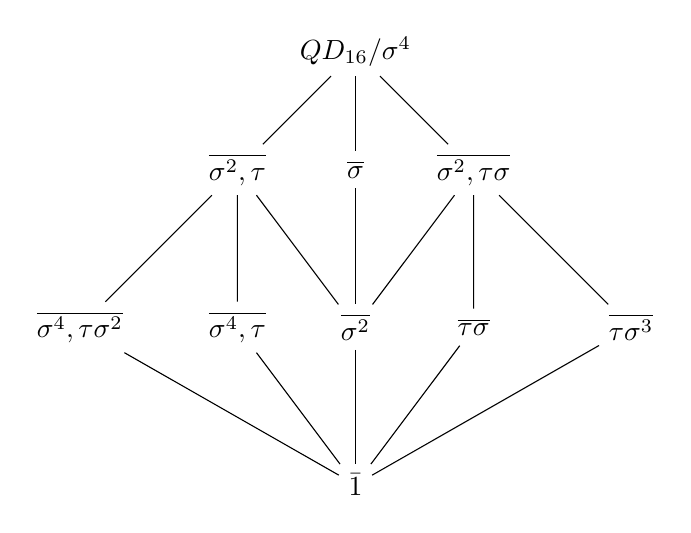
\begin{tikzpicture}
      \node (sigma4) at (0,2) {$\bar1$};
      \node (sigma2) at (0,4) {$\overline{\gen{\sigma^2}}$};
      \node (sigma4_tau) at (-1.5,4) {$\overline{\gen{\sigma^4,\tau}}$};
      \node (sigma4_tausigma2) at (-3.5,4)
      {$\overline{\gen{\sigma^4,\tau\sigma^2}}$};
      \node (tausigma) at (1.5,4) {$\overline{\gen{\tau\sigma}}$};
      \node (tausigma3) at (3.5,4) {$\overline{\gen{\tau\sigma^3}}$};
      \node (sigma) at (0,6) {$\overline{\gen{\sigma}}$};
      \node (sigma2_tau) at (-1.5,6) {$\overline{\gen{\sigma^2,\tau}}$};
      \node (sigma2_tausigma) at (1.5,6)
      {$\overline{\gen{\sigma^2,\tau\sigma}}$};
      \node (QD16) at (0,7.5) {$QD_{16}/\gen{\sigma^4}$};
      \draw (QD16) -- (sigma) -- (sigma2) -- (sigma4);
      \draw (QD16) -- (sigma2_tau) -- (sigma4_tau);
      \draw (QD16) -- (sigma2_tausigma) -- (tausigma) -- (sigma4);
      \draw (sigma2_tau) -- (sigma4_tausigma2);
      \draw (sigma2_tau) -- (sigma2) -- (sigma2_tausigma);
      \draw (sigma2_tausigma) -- (tausigma3) -- (sigma4);
      \draw (sigma4_tau) -- (sigma4);
      \draw (sigma4_tausigma2) -- (sigma4);
    \end{tikzpicture}
  \end{center}

  We can see that the dihedral group $D_8$ has the same lattice
  structure as $QD_{16}/\gen{\sigma^4}$. Since
  \begin{equation*}
    \bar\sigma^4 = \overline{\sigma^4} = \bar1,
    \qquad
    \bar\tau^2 = \overline{\tau^2} = \bar1,
  \end{equation*}
  and
  \begin{equation*}
    \bar\tau\bar\sigma = \overline{\tau\sigma}
    = \overline{\sigma^3\tau}
    = \bar\sigma^{-1}\bar\tau,
  \end{equation*}
  we see that the generators $\bar\sigma$ and $\bar\tau$ satisfy the
  same relations as $s$ and $r$ do in $D_8$. Therefore
  $QD_{16}/\gen{\sigma^4}\cong D_8$.
\end{solution}

\Exercise6 Let $M = \gen{v,u}$ be the modular group of order $16$
described in Exercise~\ref{exercise:lattice:modular16}. Prove that
$\gen{v^4}$ is normal in $M$ and use the Lattice Isomorphism Theorem
to draw the lattice of subgroups of $M/\gen{v^4}$. Which group of
order $8$ has the same lattice as this quotient? Use generators and
relations for $M/\gen{v^4}$ to decide the isomorphism type of this
group.
\begin{solution}
  Since
  \begin{equation*}
    uv^4
    = uv^{20}
    = v^4u,
  \end{equation*}
  we see that $v^4$ commutes with every element of $M$ so that
  $\gen{v^4}\trianglelefteq M$. We get the following lattice.
  \begin{center}
    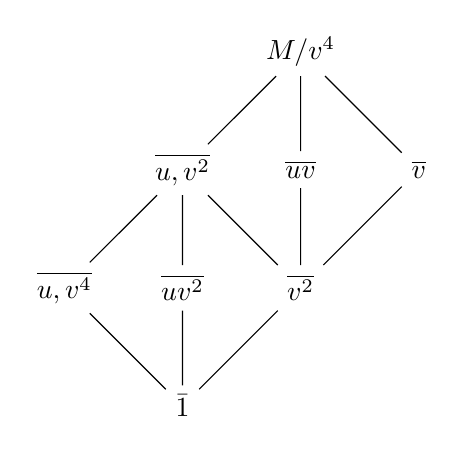
\begin{tikzpicture}[scale=0.75]
      \node (G) at (2, 2) {$M/\gen{v^4}$};
      \node (xy) at (2, 0) {$\overline{\gen{uv}}$};
      \node (y) at (4, 0) {$\overline{\gen{v}}$};
      \node (x_y2) at (0,0) {$\overline{\gen{u,v^2}}$};
      \node (y2) at (2, -2) {$\overline{\gen{v^2}}$};
      \node (x_y4) at (-2, -2) {$\overline{\gen{u, v^4}}$};
      \node (xy2) at (0, -2) {$\overline{\gen{uv^2}}$};
      \node (y4) at (0, -4) {$\bar1$};
      \draw (G) -- (x_y2) -- (x_y4);
      \draw (G) -- (y) -- (y2) -- (y4);
      \draw (G) -- (xy) -- (y2) -- (x_y2) -- (xy2) -- (y4) -- (x_y4);
    \end{tikzpicture}
  \end{center}

  Notice that the lattice looks similar to the one we constructed for
  $Z_2\times Z_4$ in Exercise~\ref{exercise:lattice:Z2-times-Z4}. We
  have
  \begin{equation*}
    \bar{u}^2 = \overline{u^2} = \bar1,
    \qquad
    \bar{v}^4 = \overline{v^4} = \bar1,
  \end{equation*}
  and
  \begin{equation*}
    \bar{u}\bar{v}
    = \overline{uv}
    = \overline{uv^{25}}
    = \overline{v^5u}
    = \bar{v}\bar{u}.
  \end{equation*}
  Since the generators $\bar{u}$ and $\bar{v}$ satisfy the same
  relations as do $a$ and $b$ in the presentation for $Z_2\times Z_4$
  (given in Exercise~\ref{exercise:lattice:Z2-times-Z4}), we conclude
  that $M/\gen{v^4}$ is isomorphic to $Z_2\times Z_4$.
\end{solution}
